\documentclass[12pt,letterpaper]{article}
\usepackage{graphicx}
\usepackage{scrextend}
\usepackage{vmargin}
\usepackage{graphicx}
\usepackage{multirow}
\usepackage[utf8]{inputenc}
\usepackage[spanish]{babel}
\usepackage{multicol}
\usepackage{enumerate}
\usepackage{float}
\usepackage{amsmath, amsthm, amssymb, amsfonts}
\usepackage[usenames]{color}
\usepackage[breaklinks=true,hidelinks]{hyperref}
\spanishdecimal{.}
\parindent=0mm
\pagestyle{empty}
\definecolor{miorange}{rgb}{0.91, 0.43, 0.0}
\begin{document}
\setmargins{2.5cm}      
{1.5cm}                     
{2cm}  
{24cm}                    
{10pt}                          
{1cm}                          
{0pt}                             
{2cm}
\begin{titlepage}
\begin{center}

\includegraphics[scale=0.40]{../../../Logos/uanl.png} 
\hspace{2.5cm}

\includegraphics[scale=0.40]{../../../Logos/fcfm.png}
\end{center}
\vspace{2cm}
\begin{center}
\textbf{
UNIVERSIDAD AUTÓNOMA DE NUEVO LEÓN\\
FACULTAD DE CIENCIAS
FÍSICO MATEMÁTICAS}\\
\vspace*{2cm}
\begin{large}
\vspace{1cm}
\large{\textbf{Aplicaciones de la Mecánica Cuántica}}\\
\textbf{Radiación de cuerpo negro}\\
Carlos Luna Criado\\
\end{large}
\vspace{3.5cm}
\begin{minipage}{0.6\linewidth}
\vspace{0.5cm}
\changefontsizes{14pt}
Nombre:\\
Giovanni Gamaliel López Padilla\\
\end{minipage}
\begin{minipage}{0.2\linewidth}
\changefontsizes{14pt}
Matricula:\\
1837522
\end{minipage}
\end{center}
\vspace{4cm}
\begin{flushright}
\today
\end{flushright}
\end{titlepage}
\begin{multicols}{2}
\section*{Introducción}
A finales del siglo XIX y comienzos del siglo XX se desarrollaron avances científicos que influyeron en la teoría cuántica de la radiación del cuerpo negro, este problema en su época fue conocido como radiación negra \cite{Planck1901}. Si una cavidad de paredes perfectamente absorbentes se mantiene a una temperatura fija T, su interior contendra energía en forma de ondas. Si la radiación está en equilibrio, ya sea en su interior como en las paredes
, entonces la tasa con la que la energía es radiada a través de cualquier área unidad es independiente de la posición  orientación de dicha superficie. El determinar y explicar la forma de la intensidad de la radiación son las componentes principales del problema del cuerpo negro. \\
A principios del siglo XX, Rayleigh \cite{LordRayleigh1900} y Jeans \cite{JHJeans1902} realizaron cálculos de la densidad de energía de la irradiancia (radiación solar de un solo rango de longitutdes de onda) emitida por un cuerpo negro. Este resultado llevo a que las investigaciones hacia un conflicto entre los resultados experimentales y física clásica. Para encontrar alguna ley de distribución clasica, los dos autores tomaron como base a la teoría electromagnética clásica para demostrar la radiación dentro de la cavidad, en donde ellos proponian que esta debia de existir en frma de ondas estacionarias con nodos en las superficies dentro del cuerpo negro. De este modo, fue encontrada 
una ecuación para el número de ondas electromagnéticas estacionaras dentro del cuerpo, esta ecuación es la siguiente: 
\begin{equation}
N(\nu)d\nu = \frac{8\pi V}{c^3} \nu^2 d\nu.
\label{N(nu)dnu}
\end{equation}
En seguida, los autores realizaron el cálculo de la energía total promedio del sistema para cada onda con frecuencia $\nu$ utilizando la ley de equipartición de la energía, llegando a la ecuación
\begin{equation}
\bar{E}=kT.
\end{equation}
Finalmente la irradiancia espectral clásica deducida por Rayleigh y Jeans es el producto del número de ondas estacionarias por unidad de volumen por la energía promedio y por la velocidad de la luz.
\begin{equation}
R_T(\nu)d\nu = \frac{8\pi \nu^2 kT}{c^2} d\nu 
\end{equation}
dando así tambien la ecuación para la densidad de energía emitida por el cuerpo negro. 
\begin{equation}
\rho_T(\nu) d\nu = \frac{8\pi \nu^2 k T}{c^3} d\nu 
\end{equation}
Al momento de comparar con los datos experimentales se percataron que para frecuencias altas (longitutdes de onda cortas) el espectro se iba hacia infinito, por lo que esto llevo a un problema, ya que esto no podia estar pasando. Esto se puede apreciar en la figura \ref{teovsexp}.
\begin{figure}[H]
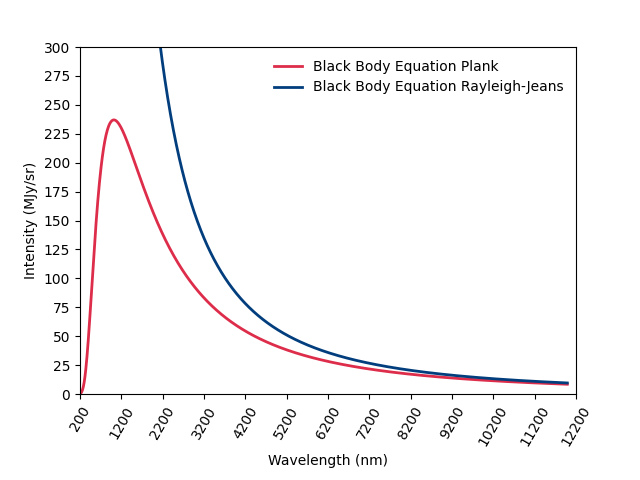
\includegraphics[scale=0.5]{../Graphics/exp_vs_teo.png}
\caption{Espectro de un cuerpo negro obtenido a partir de la ecuación de Planck y ecuación de Rayleigh-Jeans}
\label{teovsexp}
\end{figure}
Planck se percato que sucedia esto con la teoría de Rayleigh y Jeans, pero empezo a plantear que mientras más subia la frecuencia la energía media tenia que ir tendiendo a cero. 
\begin{align*}
\bar{E} &\xrightarrow[\nu \rightarrow 0]{} kT \\
\bar{E} &\xrightarrow[\nu \rightarrow \infty]{} 0 
\end{align*}
Para calcular la energía promedio es necesario determinar el valor de la integral de la ecuación \ref{emed} donde cada valor de $\bar{E}$ este pesado por su probabilidad.
\begin{equation}
\bar{E}= \frac{\int\limits_0^\infty EP(E)dE}{\int\limits_0^\infty P(E)dE} = kT
\label{emed}
\end{equation}
Donde la distribución de probabilidad $P(E)$ de Boltzmann es:
\begin{equation}
P(E)=\frac{e^{-E/kT}}{kT}
\end{equation}
La contribución de Planck surgió cuando postuló que la energía de las ondas electromagnéticas dentro de la cavidad se intercambian discretamente. De este modo, PLanck tomó los valores de $E=0,\Delta E,2\Delta E,...$,
como el conjunto de valores permitidos para la energía siendo $\Delta E$ el intervalo uniforme entre valores sucesivos.\\
En donde Planck determido una relación lineal entre $\Delta E$ y $\nu$, a partir de ajustes experimentales Planck determino el valor de la constante h $h=6.57x10^{-34} Js$, el cual es muy cercano al actual ($h=6.63x10^{-34} Js$). \\
A partir de resolver la integral \ref{emed}, Planck obtuvo la energía promedio dada por:
\begin{equation}
E(\nu) = \frac{h\nu}{e^{h\nu/kT}-1}.
\end{equation}
De este modo , el valor que se obtiene para la densidad energía espectral $\rho_T(\nu)$ usnado la energía $\bar{E}(\nu)$ es:
\begin{equation}
\rho_T(\nu) d\nu = \frac{8\pi \nu^2}{c^3} \frac{h \nu }{e^{h\ nu /kT}-1}
\end{equation}
\section*{Metodología}
En el paper \cite{Eccarelli1996} se menciona la manera en la cual se obtuvieron los datos del COBE-FIRAS, junto con la ecuación \ref{body equation}, la cual da el espectro electromagnético de un cuerpo negro con temperatura T, esto con unidades de  $W/m^2srHz$, las mediciones de COBE-FIRAS se realizaron en $Mjy/sr$, por lo que se procedio a realizar un cambio de unidades tomando en cuenta que $1 Jy /sr \rightarrow 10^{-26} W/m^2 srHz $
\begin{equation}
S(\nu,T)= \frac{2h\nu^3}{c^2} \frac{1}{e^{h\nu/kT}-1}
\label{body equation}
\end{equation}
Y la frecuencia se encuentra medida en $cm^{-1}$, por lo que se pasara de esta unidad a $Hz$ tomando en cuenta la relación $c=\lambda \nu $.
\section*{Resultados}
Al realizar el ajuste por medio de \textit{scipy} en el lenguaje  \textit{python}, se obtuvo que la temperatura a la cual se ajusta a los datos es:
\begin{equation*}
T=2.72502K
\end{equation*}
Comparando los datos con el espectro electromagnético correspondiente a este temperatura de obtiene la figura \ref{fit}
\begin{figure}[H]
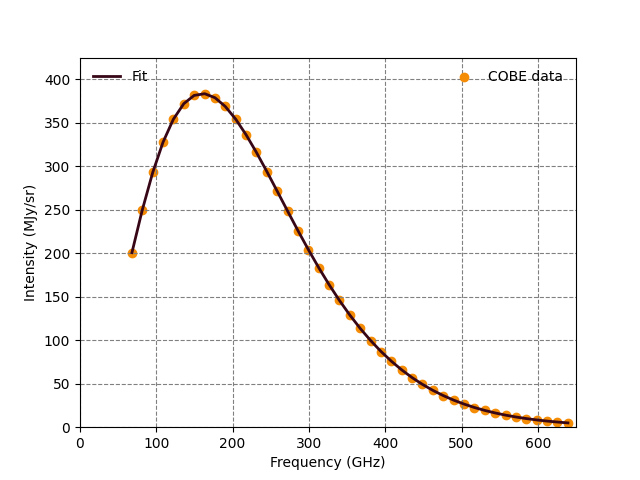
\includegraphics[scale=0.45]{../Graphics/fit.png}
\caption{Fit de los datos proporcionados por el satelite FIRAS de la misión COBE}
\label{fit}
\end{figure}
obteniendo así, un coeficiente de determinación con el ajuste de:
\begin{equation*}
R^2=0.99999972482939
\label{coef_deter}
\end{equation*}
Y para calcular la diferencia relativa entre la medición y el modelo planteado por Planck se uso la ecuación \ref{rdi} en cada punto donde tengamos el conjunto medición-modelo
\begin{equation}
RD_i = \frac{100|S_i(\nu,T)-COBE_i|}{COBE_i}
\label{rdi}
\end{equation}
Y calculando el valor medio de estos valores obtenemos que este es igual a:
\begin{equation*}
\langle RD \rangle = 0.3205\%
\end{equation*}
Realizando el calculo para diferentes temperaturas en el intervalo $[3000,6000]$ para así, calcular el espectro electromagnético correspondiente al cuerpo negro a esa temperatura obtenemos la figura \ref{dif_temp}
\begin{figure}[H]
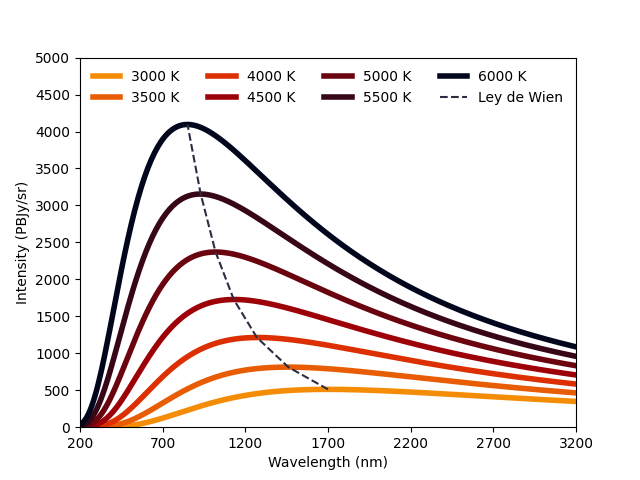
\includegraphics[scale=0.45]{../Graphics/black_body.png}
\caption{Espectro electromagnético para varias temperaturas.}
\label{dif_temp}
\end{figure}
en donde al encontrar las posiciones en que suceden los picos del espectro y unirlos se llega a formar una curva, la cual es llamada la ley de Wien. \\
Los puntos que se obtuvieron para las diferentes temperaturas son los siguientes:
\begin{table}[H]
    \centering
    \begin{tabular}{c|c}
        \hline
        Temperatura (k) & $\lambda$ (nm) \\ \hline
        3000 & 966 \\
        3500 & 828 \\ 
        4000 & 724 \\
        4500 & 644 \\ 
        5000 & 580 \\ 
        5500 & 527 \\ 
        6000 & 483 \\ \hline
    \end{tabular}
    \caption{Longitudes de onda en donde sucedio un pico en el espectro electromagnético con su respectiva temperatura del cuerpo negro}
    \label{datos de wien}
\end{table}
La ley de Wien es la siguiente:
\begin{equation}
    \lambda_{max}= \frac{2.898x10^{-3} m\cdot K}{T}
    \label{ley de wein}
\end{equation}
la cual se puede reescribir de la siguiente manera para que esta sea una liena recta:
\begin{equation}
    \lambda_{max} = 2.898x10^{-3} T^{-1}
\end{equation}
por lo que le podemos aplicar una regresión lineal a los datos de la tabla \ref{datos de wien} para asi poder nosotros calcular la constante de Wien.\\
En la figura \ref{wienfig} se observan los datos de la tabla \ref{datos de wien}, el ecuación \ref{ley de wein} y la regresión lineal que se realizó, en donde la constante de Wien calculada fue:
\begin{equation*}
    C_{Wien}= 2.8968x10^{-3}
\end{equation*}
y su diferencia relativa a la teorica es de:
\begin{equation*}
    RD_{Wien}= 0.0347 \%
\end{equation*}
por lo que se pudo llegar a comprobar la ley de Wien con estos datos.
\begin{figure}[H]
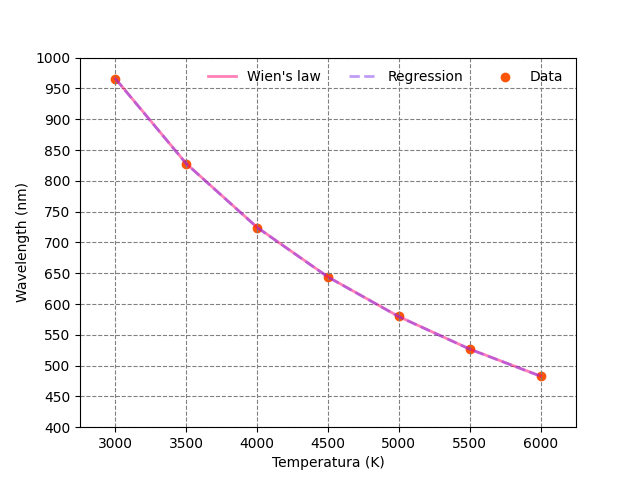
\includegraphics[scale=0.45]{../Graphics/wien_law.png}
\caption{Regresión de los datos para comprobar la ley de Wien}
\label{wienfig}
\end{figure}
Los códigos se encuentran en la sección \textbf{Código}, estos como link hacia un \textit{Github}
\section*{Conclusiones}
\begin{itemize}
\item a
\end{itemize}
\section*{Código}
\begin{itemize}
\item \href{https://github.com/giovannilopez9808/Notas_Agosto_2020/blob/master/AMC/Reto1/black_body.py}{Github - black\_body.py}\\
Este código realiza el fit de los datos de COBE guardados en el archivo  \textit{data.txt} y crea la figura \ref{fit}
\item \href{https://github.com/giovannilopez9808/Notas_Agosto_2020/blob/master/AMC/Reto1/wien_law.py}{Github - wien\_law.py}\\
Este código realiza el calculo del espectro electromagnético de un cuerpo negro para diferentes temperaturas, localiza sus picos y en base a ello opera una regresión lineal para obtener la constante de Wien.
\end{itemize}
\bibliographystyle{plain}
\bibliography{Main}
\nocite{*}
\end{multicols}
\end{document}